\documentclass{article}
\usepackage{ps}

\title{Thermal Physics 3}
\date{Due: Friday 3 October}
\usetikzlibrary{patterns}
\pagestyle{empty}
\begin{document}
\maketitle\thispagestyle{empty}
\begin{enumerate}
    \item Scientists design a particle detector which detects neutrons by measuring the temperature rise of a suitable liquid. When the neutrons enter the detector their kinetic energy is shared among the particles in liquid. 

Consider using water as the liquid in the detector. If each neutron carries \SI{3.5E-16}{\joule} of energy, calculate how many neutrons would be required to raise the temperature of \SI{1}{\kg} water by \SI{1}{\celsius}.

    \item This question is about energy changes in an ideal gas. \SI{6.0}{\g} of argon gas, molar mass \SI{0.018}{\kilogram\per\mol}, are contained at atmospheric pressure (\SI{1.0e5}{\pascal}) within a large thermally insulated container by a perfectly fitting frictionless piston, as shown below. A \SI{5.0}{\watt} electric heater is used to heat the gas for \SI{25}{\s}. The experiment is carried out twice under different conditions.
        \begin{figure}[h]
            \centering
            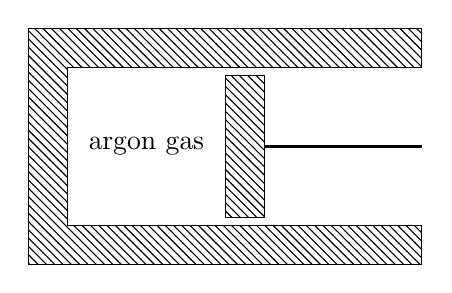
\begin{tikzpicture}
                \draw[pattern = north west lines] (5,0) -- (0,0) -- (0,3) -- (5,3) -- (5,2.5) -- (0.5,2.5) -- (0.5,0.5) -- (5,0.5) -- cycle;
                \draw[pattern = north west lines] (2.5,0.6) --(2.5,2.4) -- (3, 2.4) -- (3,0.6) -- cycle;
                \draw [very thick](3,1.5) -- (5,1.5);
                \draw (1.5,1.5) node {argon gas};
             \end{tikzpicture}
             \caption{}
        \end{figure}
        \begin{enumerate}
            \item When the piston is fixed in position, the temperature rise is \SI{30}{\K}. Calculate the heat capacity of gas using the data given.
            \item When the piston is free to move, the temperature rise is now \SI{18}{\K}. Calculate the heat capacity of the gas in this situation.
            \item Describe the difference between the two physical situations and try to account for the difference between the two values.
        \end{enumerate}
    \newpage
    \item Two cylinders \emph{A} and \emph{B} contain an ideal gas under the conditions shown in figure~\ref{fig:boxes}.        \begin{figure}[h]
            \centering
            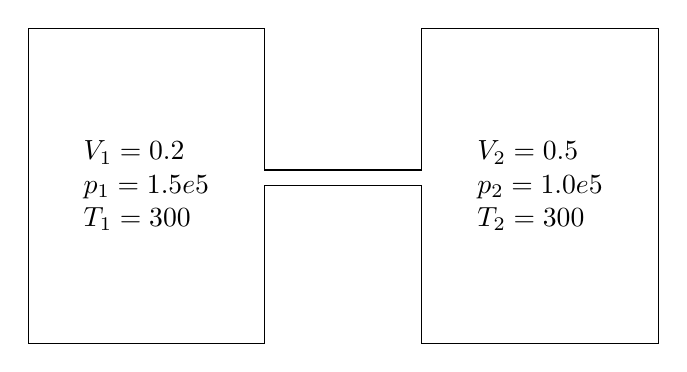
\begin{tikzpicture}
                \draw (0,0) -- (3,0) -- (3,2) -- (5,2) -- (5,0) -- (8,0) -- (8,4) -- (5,4) -- (5,2.2) -- (3,2.2) -- (3,4) -- (0,4) -- cycle;
                \draw (1.5,2) node[align=left] {$V_1 = \SI{0.2}{\m\cubed}$\\$p_1 = \SI{1.5e5}{\pascal}$\\$T_1 = \SI{300}{\K}$};
                \draw (6.5,2) node[align=left] {$V_2 = \SI{0.5}{\m\cubed}$\\$p_2 = \SI{1.0e5}{\pascal}$\\$T_2 = \SI{300}{\K}$};

            \end{tikzpicture}
            \caption{}
            \label{fig:boxes}
        \end{figure}
        \begin{enumerate}
            \item The tap is opened and steady conditions are attained. Calculate the pressure in the gas.
            \item Why is there no change in temperature?
        \end{enumerate}

    \item What must be the speed of a lead bullet if it melts when it strikes a steel slab? The initial temperature of the bullet is \SI{27}{\celsius}. The melting point of lead is \SI{327}{\celsius} and its specific heat capacity is \SI{126}{\joule\per\kg\per\celsius}. Lead requires \SI{2.1E4}{\joule\per\kg} to change from solid to liquid (called the latent heat of fusion).
    
    \item The top of the atmosphere can be considered to be at a height of 100km and the gravitational field strength can be considered constant over that distance. 
        \begin{enumerate}
            \item Estimate the average energy per air particle at the average surface temperature of \SI{15}{\celsius}.
            \item Estimate the energy required for a helium atom to reach the top of the atmosphere.
            \item Given that your answer to 2 should be greater than the answer to 1, does it mean that a helium atom can never reach the top of the atmosphere? If not, explain how it can.
            \item Calculate the ratio of the Boltzmann factor for a hydrogen atom to the Boltzmann factor for a nitrogen molecule. Hence explain why there is no atmospheric hydrogen or helium on early, but there is nitrogen.
        \end{enumerate}

\end{enumerate}

\end{document}
